% Gabarit pandoc des corrigés publiés (brut et guidé). Contenu sans marque ni nom de site.
% Compilation : lualatex (latexmk -lualatex).
% Le Markdown reste la source unique : ne pas éditer ce fichier .tex à la main.
\documentclass[11pt,a4paper]{article}

% --- Moteur, polices (Latin Modern) et langue ---------------------------------
\usepackage{iftex}
\ifLuaTeX\else\errmessage{Ce document se compile avec lualatex}\fi
\usepackage{amsmath,amssymb,mathtools}
\usepackage{fontspec}
% mathrm=sym : \mathrm prend ses glyphes dans la police mathématique (ℓ, μ, Ω), comme KaTeX.
\usepackage[math-style=TeX,bold-style=TeX,mathrm=sym]{unicode-math}
% Repli pour les glyphes absents de Latin Modern (indices et exposants Unicode,
% flèches, filets des schémas en texte, symboles) : DejaVu, puis Latin Modern Math
% (ℓ, lettres mathématiques Unicode des légendes).
\directlua{
  luaotfload.add_fallback("repliTexte", {"DejaVuSerif:mode=harf;", "DejaVuSans:mode=harf;", "file:latinmodern-math.otf:mode=harf;"})
  luaotfload.add_fallback("repliMono", {"DejaVuSansMono:mode=harf;", "DejaVuSans:mode=harf;", "file:latinmodern-math.otf:mode=harf;"})
}
\setmainfont{Latin Modern Roman}[RawFeature={fallback=repliTexte}]
\setsansfont{Latin Modern Sans}[RawFeature={fallback=repliTexte}]
\setmonofont{Latin Modern Mono}[RawFeature={fallback=repliMono}]
\setmathfont{Latin Modern Math}
\usepackage[french]{babel}
\frenchsetup{SmallCapsFigTabCaptions=false}

% --- Mise en page --------------------------------------------------------------
\usepackage[a4paper,margin=2.2cm,headheight=14pt,footskip=1.2cm]{geometry}
\usepackage{microtype}
\setlength{\emergencystretch}{4em}
\tolerance=1500
\setlength{\parindent}{0pt}
\setlength{\parskip}{0.55\baselineskip plus 2pt minus 1pt}
\usepackage{xcolor}
% Gris nommés : babel-french rend « ! » actif dans le document.
\definecolor{gris2}{gray}{0.98}
\definecolor{gris3}{gray}{0.97}
\definecolor{gris5}{gray}{0.95}
\definecolor{gris35}{gray}{0.65}
\definecolor{gris40}{gray}{0.60}
\definecolor{gris45}{gray}{0.55}
\definecolor{gris50}{gray}{0.50}
\definecolor{gris55}{gray}{0.45}
\definecolor{gris60}{gray}{0.40}
\definecolor{gris65}{gray}{0.35}
\definecolor{gris70}{gray}{0.30}
\definecolor{gris80}{gray}{0.20}
\definecolor{gris85}{gray}{0.15}
\usepackage{graphicx}
\usepackage{float}
\usepackage{caption}
\captionsetup{font=small,labelformat=empty,justification=centering}
\usepackage{booktabs,longtable,array,multirow,calc}
\usepackage{siunitx}
\sisetup{locale=FR}
\usepackage[version=4]{mhchem}
\usepackage{listings}
\usepackage{fancyhdr}
\usepackage{lastpage}
\usepackage[most]{tcolorbox}
\usepackage{enumitem}
\setlist{nosep,leftmargin=*,topsep=2pt}
\usepackage[hidelinks,unicode]{hyperref}
\usepackage{bookmark}
\hypersetup{pdftitle={Mines-Ponts MP — Maths 1 2026},pdfauthor={Rédigé par IA},pdfcreator={LaTeX},pdfsubject={Corrigé brut}}
\usepackage{xurl}

% --- Pandoc : listes, tableaux, figures ----------------------------------------
\providecommand{\passthrough}[1]{#1}
\providecommand{\tightlist}{\setlength{\itemsep}{0pt}\setlength{\parskip}{0pt}}

\makeatletter
\def\maxwidth{\ifdim\Gin@nat@width>\linewidth\linewidth\else\Gin@nat@width\fi}
\def\maxheight{\ifdim\Gin@nat@height>0.55\textheight 0.55\textheight\else\Gin@nat@height\fi}
\makeatother
\setkeys{Gin}{width=\maxwidth,height=\maxheight,keepaspectratio}
\setcounter{secnumdepth}{-\maxdimen}
\providecommand{\pandocbounded}[1]{#1}

% --- Code (listings) -----------------------------------------------------------
\lstset{
  basicstyle=\ttfamily\small,
  columns=fullflexible,
  keepspaces=true,
  breaklines=true,
  breakatwhitespace=false,
  postbreak=\mbox{\textcolor{gris50}{$\hookrightarrow$}\space},
  frame=single,
  rulecolor=\color{gris35},
  framesep=4pt,
  xleftmargin=5pt,xrightmargin=5pt,
  backgroundcolor=\color{gris3},
  keywordstyle=\bfseries,
  commentstyle=\color{gris65},
  stringstyle=\color{gris80},
  showstringspaces=false,
  tabsize=4,
  extendedchars=true,
  aboveskip=6pt,belowskip=6pt,
}

% --- Macros des corrigés (KaTeX ↔ LaTeX) ---------------------------------------
% Les corrigés sont écrits pour KaTeX : on définit ici ce que KaTeX connaît et
% que LaTeX n'a pas, sans jamais retoucher le Markdown.
\providecommand{\R}{\mathbb{R}}
\providecommand{\N}{\mathbb{N}}
\providecommand{\Z}{\mathbb{Z}}
\providecommand{\Q}{\mathbb{Q}}
\providecommand{\C}{\mathbb{C}}
\providecommand{\dd}{\mathrm{d}}
\providecommand{\llbracket}{\lBrack}
\providecommand{\rrbracket}{\rBrack}
\providecommand{\lBrace}{\lbrace}
\providecommand{\rBrace}{\rbrace}
\providecommand{\Box}{\square}
\providecommand{\Diamond}{\lozenge}
\providecommand{\varnothing}{\emptyset}
\providecommand{\argmax}{\operatorname*{arg\,max}}
\providecommand{\argmin}{\operatorname*{arg\,min}}
\renewcommand{\leq}{\leqslant}
\renewcommand{\geq}{\geqslant}

% Équation hors texte : réduite à la largeur de la ligne si elle déborde.
\newsavebox{\boiteequation}
\newcommand{\equationajustee}[1]{%
  \sbox{\boiteequation}{$\displaystyle #1$}%
  \ifdim\wd\boiteequation>\linewidth
    \[\resizebox{\linewidth}{!}{\usebox{\boiteequation}}\]%
  \else
    \[#1\]%
  \fi}

% --- Encadrés pédagogiques (sobres, lisibles en noir et blanc) -----------------
\tcbset{
  encadre/.style={
    enhanced,breakable,sharp corners,
    colback=white,colframe=gris55,
    boxrule=0.4pt,leftrule=2.2pt,
    left=6pt,right=6pt,top=3pt,bottom=3pt,
    before skip=6pt,after skip=6pt,
    fonttitle=\bfseries\small,coltitle=black,
    attach title to upper,after title={\quad},
    parbox=false,
  }
}
\newtcolorbox{indication}[1]{encadre,colframe=gris45,colback=gris2,title={Indication~#1}}
\newtcolorbox{methode}{encadre,colframe=gris70,title={Méthode}}
\newtcolorbox{piege}{encadre,colframe=gris85,boxrule=0.8pt,leftrule=2.2pt,title={Piège}}
\newtcolorbox{jury}{encadre,colframe=gris60,colback=gris5,title={Jury}}
\newtcolorbox{encadrenote}{encadre,colframe=gris40}

% --- Titres de section ---------------------------------------------------------
\usepackage{titlesec}
\titleformat{\section}{\Large\bfseries}{}{0pt}{}
\titleformat{\subsection}{\large\bfseries}{}{0pt}{}
\titleformat{\subsubsection}{\normalsize\bfseries}{}{0pt}{}
\titlespacing*{\section}{0pt}{14pt plus 4pt minus 2pt}{6pt}
\titlespacing*{\subsection}{0pt}{10pt plus 3pt minus 2pt}{4pt}
\titlespacing*{\subsubsection}{0pt}{8pt plus 2pt minus 2pt}{2pt}

% --- En-tête et pied de page ---------------------------------------------------
\pagestyle{fancy}
\fancyhf{}
\fancyhead[L]{\small\textsc{Corrigé brut} · Mines-Ponts MP}
\fancyhead[R]{\small Maths 1 2026}
\fancyfoot[L]{\footnotesize Corrigé rédigé par IA, non officiel}
\fancyfoot[R]{\footnotesize \thepage\,/\,\pageref*{LastPage}}
\renewcommand{\headrulewidth}{0.4pt}
\renewcommand{\footrulewidth}{0pt}
\fancypagestyle{plain}{\fancyhf{}\fancyfoot[R]{\footnotesize \thepage\,/\,\pageref*{LastPage}}\fancyfoot[L]{\footnotesize Corrigé rédigé par IA, non officiel}\renewcommand{\headrulewidth}{0pt}}

\begin{document}
\thispagestyle{plain}
\begin{center}
  {\small\scshape Corrigé brut}\par\smallskip
  {\LARGE\bfseries Mines-Ponts MP — Maths 1 2026\par}\medskip
  {\large Mines-Ponts · MP · Maths 1 · 2026\par}
\end{center}
\vspace{2pt}\hrule\vspace{8pt}

\emph{Corrigé rédigé par IA, non officiel. Signalez toute erreur.}

Épreuve : « Équation d'Euler-Lagrange et quelques applications ». Durée 3 h, calculatrice interdite. Toutes les normes sur les espaces de fonctions sont la norme \(\lVert\cdot\rVert_\infty\).

\hypertarget{i---lemme-fondamental-du-calcul-variationnel}{%
\section{I - Lemme fondamental du calcul variationnel}\label{i---lemme-fondamental-du-calcul-variationnel}}

Soient \(a<b\) et \(f:[a,b]\to\mathbf R\) continue.

On suppose \(\int_a^b f(x)h(x)\,\mathrm dx=0\) pour toute \(h\in\mathcal C^\infty([a,b],\mathbf R)\) vérifiant \(h(a)=h(b)=0\).

On pose
\equationajustee{\varphi(x)=\begin{cases}e^{-1/x}&\text{si }x>0,\\0&\text{si }x\le0.\end{cases}}

\hypertarget{question-1}{%
\subsection{Question 1}\label{question-1}}

Sur \(\mathbf R_+^\star\), \(x\mapsto -1/x\) est de classe \(\mathcal C^\infty\), et \(\exp\) l'est sur \(\mathbf R\).

Par composition, \(\varphi\) est de classe \(\mathcal C^\infty\) sur \(\mathbf R_+^\star\).

Montrons par récurrence sur \(n\) l'existence d'un polynôme \(P_n\) tel que \(\varphi^{(n)}(x)=P_n(1/x)e^{-1/x}\) pour tout \(x>0\).

\begin{itemize}
\tightlist
\item
  \(n=0\) : \(P_0=1\) convient.
\item
  Si \(P_n\) convient, alors pour \(x>0\), en dérivant le produit (la dérivée de \(x\mapsto P_n(1/x)\) est \(x\mapsto-\frac1{x^2}P_n'(1/x)\)) :
  \equationajustee{\begin{aligned}
  \varphi^{(n+1)}(x)&=-\frac1{x^2}P_n'\!\left(\frac1x\right)e^{-1/x}+\frac1{x^2}P_n\!\left(\frac1x\right)e^{-1/x}\\
  &=P_{n+1}\!\left(\frac1x\right)e^{-1/x},
  \end{aligned}}
  avec \(P_{n+1}=X^2\,(P_n-P_n')\), qui est un polynôme.
\end{itemize}

\equationajustee{\boxed{\begin{aligned}{}&P_0=1,\\
&P_{n+1}=X^2(P_n-P_n'),\\
&\varphi^{(n)}(x)=P_n\!\left(\tfrac1x\right)e^{-1/x}\ \ (x>0).
\end{aligned}}}

\hypertarget{question-2}{%
\subsection{Question 2}\label{question-2}}

\textbf{Lemme.} Pour tout polynôme \(P\), \(P(1/x)e^{-1/x}\to0\) quand \(x\to0^+\). En effet, avec \(t=1/x\to+\infty\), \(P(t)e^{-t}\to0\) par croissances comparées.

Montrons par récurrence sur \(n\) : « \(\varphi\) est de classe \(\mathcal C^n\) sur \(\mathbf R\) et \(\varphi^{(n)}\) est nulle sur \(\mathbf R_-\) ».

\begin{itemize}
\item
  \(n=0\) : \(\varphi\) est continue sur \(\mathbf R_-^\star\) (nulle) et sur \(\mathbf R_+^\star\).

  En \(0\), \(\varphi(x)\to0=\varphi(0)\) à gauche, et à droite par le lemme avec \(P=1\).

  Donc \(\varphi\) est continue sur \(\mathbf R\), nulle sur \(\mathbf R_-\).
\item
  Hérédité : supposons la propriété vraie au rang \(n\) et posons \(g=\varphi^{(n)}\). Vérifions les hypothèses du théorème de la limite de la dérivée (prolongement de la classe \(\mathcal C^1\)) :

  \begin{itemize}
  \tightlist
  \item
    \(g\) est \textbf{continue sur \(\mathbf R\)}, en particulier en \(0\) (hypothèse de récurrence) ;
  \item
    \(g\) est de classe \(\mathcal C^1\) sur \(\mathbf R^\star\) : \(g'=0\) sur \(\mathbf R_-^\star\),
    et \(g'(x)=P_{n+1}(1/x)e^{-1/x}\) sur \(\mathbf R_+^\star\) (Q1) ;
  \item
    \(g'(x)\to0\) quand \(x\to0^-\) (fonction nulle) et quand \(x\to0^+\) (lemme).
  \end{itemize}

  Le théorème donne : \(g\) est dérivable en \(0\), \(g'(0)=0\), et \(g'\) est continue en \(0\).

  Ainsi \(\varphi\) est de classe \(\mathcal C^{n+1}\) sur \(\mathbf R\) et \(\varphi^{(n+1)}\) est nulle sur \(\mathbf R_-\).
\end{itemize}

\textbf{Donc \(\varphi\) est de classe \(\mathcal C^\infty\) sur \(\mathbf R\)}, avec \(\varphi^{(n)}(0)=0\) pour tout \(n\).

\hypertarget{question-3}{%
\subsection{Question 3}\label{question-3}}

Posons, pour \(x\in\mathbf R\),
\equationajustee{\boxed{\psi_{c,d}(x)=\varphi(x-c)\,\varphi(d-x).}}

\begin{itemize}
\tightlist
\item
  Par composition avec des fonctions affines et produit, \(\psi_{c,d}\) est de classe \(\mathcal C^\infty\) sur \(\mathbf R\) (Q2).
\item
  Si \(c<x<d\) : \(x-c>0\) et \(d-x>0\), donc \(\psi_{c,d}(x)=e^{-1/(x-c)}e^{-1/(d-x)}>0\).
\item
  Si \(x\le c\), \(\varphi(x-c)=0\) ; si \(x\ge d\), \(\varphi(d-x)=0\). Donc \(\psi_{c,d}\) est nulle sur \(\mathbf R\setminus\,]c,d[\).
\end{itemize}

\hypertarget{question-4}{%
\subsection{Question 4}\label{question-4}}

Raisonnons par l'absurde : supposons qu'il existe \(x_0\in\,]a,b[\) tel que \(f(x_0)\ne0\).

Quitte à changer \(f\) en \(-f\) (l'hypothèse est inchangée), \(f(x_0)>0\).

Par continuité de \(f\) en \(x_0\), il existe \(\delta>0\) tel que \([x_0-\delta,x_0+\delta]\subset\,]a,b[\) et \(f\ge f(x_0)/2>0\) sur ce segment.

Posons \(c=x_0-\delta\), \(d=x_0+\delta\), et \(h=\psi_{c,d}\) restreinte à \([a,b]\).

Alors \(h\) est de classe \(\mathcal C^\infty\), et \(h(a)=h(b)=0\) puisque \(a,b\notin\,]c,d[\). Donc \(\int_a^b fh=0\).

\begin{figure}[H]
\centering
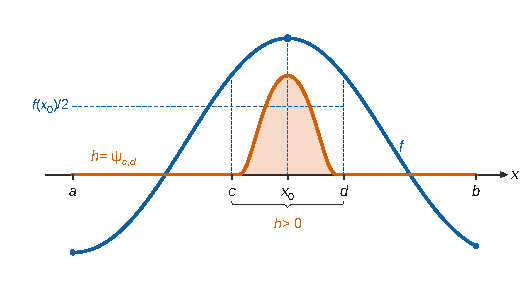
\includegraphics{figures/q4-fonction-test-bosse.pdf}
\caption*{Figure 1 --- Fonction test h = ψ\_\{c,d\} : strictement positive pour c
\textless{} x \textless{} d, nulle ailleurs, portée par un segment
autour de x₀ où f ≥ f(x₀)/2 \textgreater{} 0}
\end{figure}

Or \(fh\) est nulle hors de \(]c,d[\), d'où \(\int_a^b fh=\int_c^d fh\). C'est l'intégrale d'une fonction continue, positive sur \([c,d]\) et strictement positive en \(x_0\).

Une fonction continue positive d'intégrale nulle sur un segment étant nulle, \(\int_c^d fh>0\). Contradiction.

Donc \(f\) est nulle sur \(]a,b[\), puis sur \([a,b]\) par continuité en \(a\) et \(b\) :
\equationajustee{\boxed{f=0\ \text{sur}\ [a,b].}}

\emph{La preuve n'utilise que des fonctions test \(\psi_{c,d}\) avec \(a<c<d<b\) ; ce point resservira en Q12.}

\hypertarget{ii---uxe9quation-deuler-lagrange}{%
\section{II - Équation d'Euler-Lagrange}\label{ii---uxe9quation-deuler-lagrange}}

\textbf{Convention.} Les questions 7 à 9 font intervenir \(\partial f/\partial y\), \(\partial f/\partial z\) et \(\frac{\mathrm d}{\mathrm dx}\frac{\partial f}{\partial z}\) jusqu'aux bornes de \([x_A,x_B]\).

Or \(f\) n'est supposée de classe \(\mathcal C^2\) que sur l'ouvert \(]x_A,x_B[\times U\times V\).

On lit l'énoncé ainsi : les dérivées partielles de \(f\) d'ordre au plus \(2\) se prolongent continûment à \([x_A,x_B]\times U\times V\).

C'est le cas dans toutes les applications (parties III à V), où \(f\) ne dépend pas de \(x\) et est de classe \(\mathcal C^\infty\) sur \(\mathbf R\times U\times V\).

\hypertarget{question-5}{%
\subsection{Question 5}\label{question-5}}

Soit \(y\in\mathcal C\). L'application \(\Gamma:x\mapsto(x,y(x),y'(x))\) est continue sur \([x_A,x_B]\), car \(y\) est de classe \(\mathcal C^1\).

Elle est à valeurs dans \([x_A,x_B]\times U\times V\) par définition de \(\mathcal C\). Comme \(f\) est continue sur cet ensemble, \(f\circ\Gamma\) est continue sur le segment \([x_A,x_B]\), donc intégrable : \textbf{\(T(y)\) existe}.

\hypertarget{question-6}{%
\subsection{Question 6}\label{question-6}}

Pour tout \(\varepsilon\), \(y_\varepsilon=z_0+\varepsilon\eta\) est de classe \(\mathcal C^2\). De plus \(y_\varepsilon(x_A)=y_0\) et \(y_\varepsilon(x_B)=y_1\) car \(\eta(x_A)=\eta(x_B)=0\).

Il reste à trouver \(\alpha>0\) tel que, pour \(\lvert\varepsilon\rvert<\alpha\) et tout \(x\in[x_A,x_B]\), \(y_\varepsilon(x)\in U\) et \(y_\varepsilon'(x)\in V\).

\begin{figure}[H]
\centering
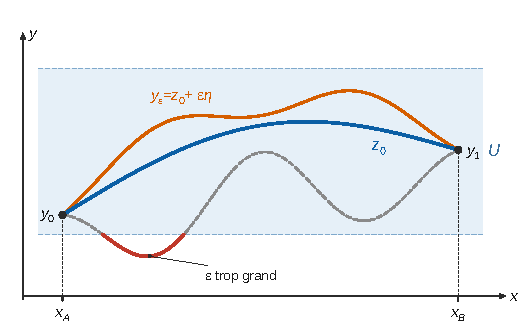
\includegraphics{figures/q6-perturbation-admissible.pdf}
\caption*{Figure 2 --- Perturbation y\_ε = z₀ + εη à extrémités fixes : pour
\textbar ε\textbar{} petit le graphe reste dans U, un ε trop grand peut
l'en faire sortir}
\end{figure}

Par l'absurde : sinon, pour tout \(n\ge1\), il existe \(\varepsilon_n\in\,]-\frac1n,\frac1n[\) et \(x_n\in[x_A,x_B]\) tels que
\equationajustee{z_0(x_n)+\varepsilon_n\eta(x_n)\notin U\qquad\text{ou}\qquad z_0'(x_n)+\varepsilon_n\eta'(x_n)\notin V.}
L'un des deux cas se produit pour une infinité d'indices ; quitte à extraire, c'est toujours le premier. Le second se traite de même en remplaçant \((z_0,\eta,U)\) par \((z_0',\eta',V)\), ces fonctions étant continues.

La suite \((x_n)\) est bornée : par Bolzano-Weierstrass, une sous-suite \((x_{\sigma(n)})\) converge vers \(\ell\in[x_A,x_B]\) (segment fermé).

Comme \(z_0\) est continue, \(\eta\) bornée sur le segment et \(\varepsilon_{\sigma(n)}\to0\),
\equationajustee{u_n=z_0(x_{\sigma(n)})+\varepsilon_{\sigma(n)}\eta(x_{\sigma(n)})\longrightarrow z_0(\ell).}
Or \(u_n\in\mathbf R\setminus U\), fermé puisque \(U\) est ouvert ; par caractérisation séquentielle, \(z_0(\ell)\notin U\). C'est absurde car \(z_0\in\mathcal C\).

\textbf{Il existe donc \(\alpha>0\) tel que \(y_\varepsilon\in\mathcal C\) pour tout \(\varepsilon\in\,]-\alpha,\alpha[\).}

\hypertarget{question-7}{%
\subsection{Question 7}\label{question-7}}

Posons \(F(\varepsilon,x)=f(x,y_\varepsilon(x),y_\varepsilon'(x))\) pour \(\lvert\varepsilon\rvert<\alpha\) et \(x\in[x_A,x_B]\). Fixons \(\beta\in\,]0,\alpha[\) et travaillons sur \(J=[-\beta,\beta]\).

\begin{itemize}
\item
  Pour \(\varepsilon\in J\), \(x\mapsto F(\varepsilon,x)\) est continue sur le segment (Q5), donc intégrable.
\item
  Pour \(x\) fixé, \(\varepsilon\mapsto(x,\allowbreak z_0(x)+\varepsilon\eta(x),\allowbreak z_0'(x)+\varepsilon\eta'(x))\) est affine, à valeurs dans \([x_A,x_B]\times U\times V\), où \(f\) est de classe \(\mathcal C^1\).

  Par la règle de la chaîne, \(\varepsilon\mapsto F(\varepsilon,x)\) est de classe \(\mathcal C^1\) et
  \equationajustee{\frac{\partial F}{\partial\varepsilon}(\varepsilon,x)=\eta(x)\frac{\partial f}{\partial y}(x,y_\varepsilon(x),y_\varepsilon'(x))+\eta'(x)\frac{\partial f}{\partial z}(x,y_\varepsilon(x),y_\varepsilon'(x)),}
  fonction continue de \(x\) à \(\varepsilon\) fixé.
\item
  Domination : \(\Phi:(\varepsilon,\allowbreak x)\mapsto(x,\allowbreak y_\varepsilon(x),\allowbreak y_\varepsilon'(x))\) est continue sur le compact \(J\times[x_A,x_B]\).

  Donc \(K=\Phi(J\times[x_A,x_B])\) est un compact, inclus dans \([x_A,x_B]\times U\times V\) (Q6).

  Les fonctions continues \(\partial f/\partial y\) et \(\partial f/\partial z\) y sont bornées par un réel \(M\).

  C'est ici que sert la convention : les dérivées partielles doivent être continues jusqu'aux bornes du segment.

  D'où, pour \(\varepsilon\in J\) et \(x\in[x_A,x_B]\),
  \equationajustee{\left\lvert\frac{\partial F}{\partial\varepsilon}(\varepsilon,x)\right\rvert\le M\big(\lVert\eta\rVert_\infty+\lVert\eta'\rVert_\infty\big),}
  constante indépendante de \(\varepsilon\), intégrable sur le segment.
\end{itemize}

Par le théorème de dérivation sous le signe intégral, \(\varphi\) est de classe \(\mathcal C^1\) sur \(]-\beta,\beta[\) pour tout \(\beta<\alpha\), donc sur \(]-\alpha,\alpha[\), et
\equationajustee{\boxed{\varphi'(\varepsilon)=\int_{x_A}^{x_B}\left(\eta(x)\frac{\partial f}{\partial y}(x,y_\varepsilon(x),y_\varepsilon'(x))+\eta'(x)\frac{\partial f}{\partial z}(x,y_\varepsilon(x),y_\varepsilon'(x))\right)\mathrm dx.}}

\hypertarget{question-8}{%
\subsection{Question 8}\label{question-8}}

Traitons un minimum local (le maximum est symétrique) : il existe \(r>0\) tel que \(T(y)\ge T(z_0)\) pour tout \(y\in\mathcal C\) avec \(\lVert y-z_0\rVert_\infty\le r\).

Soit \(\lvert\varepsilon\rvert<\min\big(\alpha,\allowbreak \ r/(\lVert\eta\rVert_\infty+1)\big)\). Alors \(y_\varepsilon\in\mathcal C\) et
\equationajustee{\lVert y_\varepsilon-z_0\rVert_\infty=\lvert\varepsilon\rvert\,\lVert\eta\rVert_\infty\le r,}
donc \(\varphi(\varepsilon)=T(y_\varepsilon)\ge T(z_0)=\varphi(0)\).

Ainsi \(\varphi\) a un minimum local en \(0\). Or en un extremum d'une fonction dérivable sur un intervalle ouvert, la dérivée s'annule ; \(0\) est intérieur à \(]-\alpha,\alpha[\) et \(\varphi\) y est dérivable (Q7) : \(\varphi'(0)=0\).

Posons \(w(x)=\frac{\partial f}{\partial z}(x,z_0(x),z_0'(x))\). Avec \(y_{\varepsilon=0}=z_0\), Q7 donne
\equationajustee{\int_{x_A}^{x_B}\left(\eta\,\frac{\partial f}{\partial y}(x,z_0,z_0')+\eta'\,w\right)\mathrm dx=0.}

L'application \(x\mapsto(x,z_0(x),z_0'(x))\) est de classe \(\mathcal C^1\), car \(z_0\) est de classe \(\mathcal C^2\).

De plus \(\partial f/\partial z\) est de classe \(\mathcal C^1\), car \(f\) est de classe \(\mathcal C^2\).

Donc \(w\) est de classe \(\mathcal C^1\) sur \([x_A,x_B]\).

Sa dérivée est \(w'=\frac{\mathrm d}{\mathrm dx}\left(\frac{\partial f}{\partial z}(x,\allowbreak z_0,\allowbreak z_0')\right)\).

L'intégration par parties (\(\eta\) et \(w\) de classe \(\mathcal C^1\)) donne, car \(\eta(x_A)=\eta(x_B)=0\) :
\equationajustee{\begin{aligned}
\int_{x_A}^{x_B}\eta'w&=\big[\eta w\big]_{x_A}^{x_B}-\int_{x_A}^{x_B}\eta w'\\
&=-\int_{x_A}^{x_B}\eta w'.
\end{aligned}}
D'où
\equationajustee{\boxed{\int_{x_A}^{x_B}\left(\frac{\partial f}{\partial y}(x,z_0(x),z_0'(x))-\frac{\mathrm d}{\mathrm dx}\left(\frac{\partial f}{\partial z}(x,z_0(x),z_0'(x))\right)\right)\eta(x)\,\mathrm dx=0.}}

\hypertarget{question-9}{%
\subsection{Question 9}\label{question-9}}

Posons \(E:x\mapsto\frac{\partial f}{\partial y}(x,\allowbreak z_0(x),\allowbreak z_0'(x))-w'(x)\). Elle est continue sur \([x_A,x_B]\) (composée de fonctions continues, et \(w\) de classe \(\mathcal C^1\)).

Toute \(h\in\mathcal C^\infty([x_A,x_B],\mathbf R)\) nulle en \(x_A\) et \(x_B\) est de classe \(\mathcal C^2\), donc admissible comme \(\eta\) en Q8 : \(\int_{x_A}^{x_B}Eh=0\).

Les hypothèses de Q4 sont donc réunies (avec \(a=x_A\), \(b=x_B\) et \(E\) continue à la place de \(f\)) : \(E=0\), soit
\equationajustee{\boxed{\forall x\in[x_A,x_B],\quad \frac{\partial f}{\partial y}(x,z_0(x),z_0'(x))-\frac{\mathrm d}{\mathrm dx}\left(\frac{\partial f}{\partial z}(x,z_0(x),z_0'(x))\right)=0.}}

\emph{Remarque.} Sans la convention de prolongement, on obtient la même équation sur \(]x_A,x_B[\) en prenant \(\eta=\psi_{c,d}\) avec \(x_A<c<d<x_B\). En effet, \(\varphi(\varepsilon)\) ne diffère alors d'une constante que par une intégrale sur \([c,d]\), où tout est de classe \(\mathcal C^2\), et la preuve de Q4 n'utilise que ces fonctions test.

\hypertarget{question-10}{%
\subsection{Question 10}\label{question-10}}

Posons, pour \(x\in\,]x_A,x_B[\), \(H(x)=f(x,z_0(x),z_0'(x))-z_0'(x)\,w(x)\).

Comme \(f\) est de classe \(\mathcal C^2\) sur \(]x_A,x_B[\times U\times V\) et \(x\mapsto(x,z_0,z_0')\) de classe \(\mathcal C^1\), \(H\) est dérivable (règle de la chaîne).

En abrégeant les arguments \((x,z_0(x),z_0'(x))\) :
\equationajustee{\begin{aligned}
H'&=\frac{\partial f}{\partial x}+z_0'\frac{\partial f}{\partial y}+z_0''\frac{\partial f}{\partial z}-z_0''w-z_0'w'\\
&=\frac{\partial f}{\partial x}+z_0'\left(\frac{\partial f}{\partial y}-w'\right),
\end{aligned}}
puisque \(w=\frac{\partial f}{\partial z}(x,z_0,z_0')\).

Le premier terme est nul par hypothèse, le second par l'équation d'Euler-Lagrange (Q9). Donc \(H'=0\) sur l'intervalle \(]x_A,x_B[\), et \(H\) y est constante :
\equationajustee{\boxed{\exists C\in\mathbf R,\ \forall x\in\,]x_A,x_B[,\quad f(x,z_0(x),z_0'(x))-z_0'(x)\frac{\partial f}{\partial z}(x,z_0(x),z_0'(x))=C.}}

\hypertarget{iii---le-chemin-le-plus-court-est-la-ligne-droite}{%
\section{III - Le chemin le plus court est la ligne droite !}\label{iii---le-chemin-le-plus-court-est-la-ligne-droite}}

\hypertarget{question-11}{%
\subsection{Question 11}\label{question-11}}

On applique la partie II avec \(U=V=\mathbf R\), les valeurs aux bords \(y_A\), \(y_B\), et
\equationajustee{f:(x,y,z)\in[x_A,x_B]\times\mathbf R\times\mathbf R\longmapsto\sqrt{1+z^2},}
restriction d'une fonction de classe \(\mathcal C^\infty\) sur \(\mathbf R^3\) (car \(1+z^2>0\)).

L'ensemble \(\mathcal C\) est celui de la partie II, et un extremum de \(T\) est en particulier un extremum local. On a \(\partial f/\partial x=0\) et \(\partial f/\partial z=z/\sqrt{1+z^2}\).

L'identité de Beltrami donne \(C\in\mathbf R\) tel que, pour \(x\in\,]x_A,x_B[\),
\equationajustee{\begin{aligned}
C&=\sqrt{1+y_0'^2}-\frac{y_0'^2}{\sqrt{1+y_0'^2}}\\
&=\frac{1}{\sqrt{1+y_0'(x)^2}}.
\end{aligned}}
Donc \(C>0\) (inverse d'une racine strictement positive) et \(y_0'(x)^2=\frac1{C^2}-1=:k^2\) avec \(k\ge0\).

Ainsi \(y_0'\) est à valeurs dans \(\{-k,k\}\) sur \(]x_A,x_B[\). Comme \(y_0'\) est continue, \(y_0'(]x_A,x_B[)\) est un intervalle (théorème des valeurs intermédiaires) contenu dans \(\{-k,k\}\), donc un singleton.

Donc \(y_0'\) est constante, égale à \(m\), sur \(]x_A,x_B[\), puis sur \([x_A,x_B]\) par continuité. Ainsi \(y_0(x)=mx+p\) :
\equationajustee{\boxed{y_0\ \text{est affine :}\quad y_0(x)=y_A+\frac{y_B-y_A}{x_B-x_A}(x-x_A).}}

\hypertarget{iv---le-chemin-le-plus-rapide-est-la-cyclouxefde}{%
\section{IV - Le chemin le plus rapide est la cycloïde}\label{iv---le-chemin-le-plus-rapide-est-la-cyclouxefde}}

\hypertarget{question-12}{%
\subsection{Question 12}\label{question-12}}

Posons \(f(x,y,z)=\sqrt{(1+z^2)/y}\), de classe \(\mathcal C^\infty\) sur \(\mathbf R\times\mathbf R_+^\star\times\mathbf R\). On a \(\frac{\partial f}{\partial x}=0\) et
\equationajustee{\frac{\partial f}{\partial z}(x,y,z)=\frac{z}{\sqrt y\,\sqrt{1+z^2}}.}

\textbf{Équation d'Euler-Lagrange sur \(]x_A,x_B[\).} L'ensemble \(\mathcal C\) de cette partie n'est pas exactement de la forme de la partie II : la condition \(y'<0\) ne porte que sur \(]x_A,x_B]\), et \(y_0\) ne minimise \(T\) que sur cet ensemble. On refait donc l'argument de variation.

Soient \(x_A<c<d<x_B\) et \(\eta=\psi_{c,d}\) (restreinte), de classe \(\mathcal C^\infty\), nulle hors de \(]c,d[\). Posons
\equationajustee{\begin{aligned}
m&=\min_{[x_A,x_B]}y_0>0,\\
\mu&=-\max_{[c,d]}y_0'>0
\end{aligned}}
(fonctions continues sur des segments, et \([c,d]\subset\,]x_A,x_B]\)), puis
\equationajustee{\alpha=\min\left(\frac{m}{\lVert\eta\rVert_\infty+1},\ \frac{\mu}{\lVert\eta'\rVert_\infty+1}\right).}

Pour \(\lvert\varepsilon\rvert<\alpha\), \(y_\varepsilon=y_0+\varepsilon\eta\) est de classe \(\mathcal C^2\) et a les bonnes valeurs aux bords. De plus :

\begin{itemize}
\tightlist
\item
  \(y_\varepsilon\ge m-\lvert\varepsilon\rvert\lVert\eta\rVert_\infty>0\) ;
\item
  \(y_\varepsilon'=y_0'<0\) sur \(]x_A,x_B]\setminus[c,d]\) ;
\item
  \(y_\varepsilon'\le-\mu+\lvert\varepsilon\rvert\lVert\eta'\rVert_\infty<0\) sur \([c,d]\).
\end{itemize}

Donc \(y_\varepsilon\in\mathcal C\), et \(\varphi(\varepsilon)=T(y_\varepsilon)\ge T(y_0)=\varphi(0)\) sur \(]-\alpha,\alpha[\).

Les preuves de Q7 et Q8 s'appliquent mot pour mot : le compact \(K\) est inclus dans \(\mathbf R\times\mathbf R_+^\star\times\mathbf R\), où \(f\) est \(\mathcal C^\infty\). Elles donnent \(\int_{x_A}^{x_B}E\,\psi_{c,d}=0\), où \(E=\frac{\partial f}{\partial y}(x,\allowbreak y_0,\allowbreak y_0')-\frac{\mathrm d}{\mathrm dx}\frac{\partial f}{\partial z}(x,\allowbreak y_0,\allowbreak y_0')\) est continue.

Comme la preuve de Q4 n'utilise que ces fonctions test, \(E=0\) sur \([x_A,x_B]\).

\textbf{Intégrale première.} Le calcul de Q10 n'utilise que \(\partial f/\partial x=0\) et l'équation d'Euler-Lagrange sur \(]x_A,x_B[\). Il fournit \(K\in\mathbf R\) tel que, pour \(x\in\,]x_A,x_B[\),
\equationajustee{\begin{aligned}
K&=\sqrt{\frac{1+y_0'^2}{y_0}}-\frac{y_0'^2}{\sqrt{y_0}\sqrt{1+y_0'^2}}\\
&=\frac{1}{\sqrt{y_0(x)\big(1+y_0'(x)^2\big)}}.
\end{aligned}}
Donc \(K>0\) et \(y_0(x)(1+y_0'(x)^2)=1/K^2\) sur \(]x_A,x_B[\), puis sur \([x_A,x_B]\) par continuité. Avec \(C=1/K^2>0\) :
\equationajustee{\boxed{\forall x\in[x_A,x_B],\quad y_0(x)\big(1+y_0'(x)^2\big)=C.}}

\emph{(Si l'on admet que la partie II s'applique avec \(U=\mathbf R_+^\star\), le résultat est une application directe de l'identité de Beltrami ; l'argument ci-dessus justifie cette application.)}

Dans la suite, \(C=2\).

\hypertarget{question-13}{%
\subsection{Question 13}\label{question-13}}

\(\operatorname{cotan}=\cos/\sin\) est définie là où \(\sin\) ne s'annule pas :
\equationajustee{\boxed{\mathcal D_{\operatorname{cotan}}=\mathbf R\setminus\pi\mathbf Z.}}

Sur \(]0,\pi[\), \(\operatorname{cotan}\) est dérivable et
\equationajustee{\begin{aligned}
\operatorname{cotan}'(x)&=\frac{-\sin^2x-\cos^2x}{\sin^2x}\\
&=-\frac1{\sin^2x}<0.
\end{aligned}}
Elle est continue et strictement décroissante.

Quand \(x\to0^+\), \(\cos x\to1\) et \(\sin x\to0^+\), donc \(\operatorname{cotan}x\to+\infty\).

Quand \(x\to\pi^-\), \(\cos x\to-1\) et \(\sin x\to0^+\), donc \(\operatorname{cotan}x\to-\infty\).

Par le théorème de la bijection (fonction continue et strictement monotone sur un intervalle), \textbf{\(\operatorname{cotan}\) réalise une bijection de \(]0,\pi[\) sur \(\mathbf R\)}. On note \(\operatorname{arccotan}:\mathbf R\to\,]0,\pi[\) sa réciproque, continue et strictement décroissante.

Comme \(\operatorname{cotan}'\) ne s'annule pas sur \(]0,\pi[\), \(\operatorname{arccotan}\) est dérivable en tout point de \(\mathbf R\). Soit \(t\in\mathbf R\) et \(u=\operatorname{arccotan}t\) ; on a
\equationajustee{\sin^2u=\frac1{1+\operatorname{cotan}^2u}=\frac1{1+t^2}.}
D'où
\equationajustee{\boxed{\begin{aligned}
\forall t\in\mathbf R,\quad \operatorname{arccotan}'(t)&=-\sin^2(\operatorname{arccotan}t)\\
&=-\frac{1}{1+t^2}.
\end{aligned}}}

\hypertarget{question-14}{%
\subsection{Question 14}\label{question-14}}

Soit \(x\in[x_A,x_B]\) et \(u=\theta(x)/2=\operatorname{arccotan}(y_0'(x))\in\,]0,\pi[\). Alors \(\sin u\ne0\), \(\operatorname{cotan}u=y_0'(x)\) et
\equationajustee{\begin{aligned}
1-\cos\theta(x)&=1-\cos(2u)\\
&=2\sin^2u\\
&=\frac{2}{1+\operatorname{cotan}^2u}\\
&=\frac{2}{1+y_0'(x)^2}.
\end{aligned}}
Or Q12 avec \(C=2\) donne \(y_0(x)=\dfrac{2}{1+y_0'(x)^2}\). Donc
\equationajustee{\boxed{\forall x\in[x_A,x_B],\quad y_0(x)=1-\cos\theta(x).}}

\hypertarget{question-15}{%
\subsection{Question 15}\label{question-15}}

\(y_0'\) est de classe \(\mathcal C^1\) et \(\operatorname{arccotan}\) aussi (dérivée continue, Q13), donc \(\theta\) est de classe \(\mathcal C^1\) sur \([x_A,x_B]\). En dérivant Q14 :
\equationajustee{\begin{aligned}
y_0'(x)&=\theta'(x)\sin\theta(x)\\
&=2\theta'(x)\sin\frac{\theta(x)}2\cos\frac{\theta(x)}2.
\end{aligned}}
Par ailleurs, par définition de \(\theta\),
\equationajustee{y_0'(x)=\operatorname{cotan}\frac{\theta(x)}2=\frac{\cos(\theta(x)/2)}{\sin(\theta(x)/2)}.}

Soit \(x\in\,]x_A,x_B]\) : \(y_0'(x)<0\) et \(\sin\frac{\theta(x)}2>0\) imposent \(\cos\frac{\theta(x)}2<0\), en particulier non nul.

En égalant les deux expressions, en multipliant par \(\sin\frac{\theta(x)}2\) et en simplifiant par \(\cos\frac{\theta(x)}2\) :
\equationajustee{\begin{aligned}
1&=2\theta'(x)\sin^2\frac{\theta(x)}2\\
&=\theta'(x)\big(1-\cos\theta(x)\big).
\end{aligned}}

Posons \(\Lambda(x)=\theta(x)-\sin\theta(x)-x\), de classe \(\mathcal C^1\) sur \([x_A,x_B]\). Sur \(]x_A,x_B[\), \(\Lambda'=\theta'(1-\cos\theta)-1=0\).

Donc \(\Lambda\) y est constante, égale à \(-c\), puis sur \([x_A,x_B]\) par continuité. Ainsi
\equationajustee{\boxed{\exists c\in\mathbf R,\ \forall x\in[x_A,x_B],\quad x=\theta(x)-\sin\theta(x)+c.}}

La courbe de \(y_0\) est donc l'arc \(\theta\mapsto(\theta-\sin\theta+c,\ 1-\cos\theta)\), \(\theta\in\theta([x_A,x_B])\) : un arc de cycloïde (avec \(\theta(x)\in\,]\pi,2\pi[\) pour \(x\in\,]x_A,x_B]\)).

\begin{figure}[H]
\centering
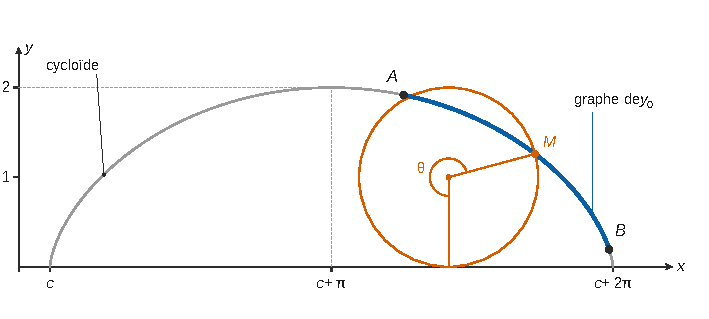
\includegraphics{figures/q15-arc-cycloide.pdf}
\caption*{Figure 3 --- Le graphe de y₀ (de A à B) est un arc de la cycloïde θ ↦ (θ
− sin θ + c, 1 − cos θ), décrite par un point M d'un cercle de rayon 1
qui roule}
\end{figure}

\hypertarget{v---une-application-uxe0-une-structure-optimale-la-catuxe9nouxefde}{%
\section{V - Une application à une structure optimale : la caténoïde}\label{v---une-application-uxe0-une-structure-optimale-la-catuxe9nouxefde}}

\hypertarget{question-16}{%
\subsection{Question 16}\label{question-16}}

Le facteur \(2\pi>0\) ne change pas les minimiseurs : \(y_0\) minimise \(y\mapsto\int_0^1 y\sqrt{1+y'^2}\) sur \(\mathcal C\).

C'est l'ensemble de la partie II avec \(x_A=0\), \(x_B=1\), \(U=V=\mathbf R\) et les valeurs \(1\), \(1\) aux bords.

On prend \(f(x,y,z)=y\sqrt{1+z^2}\), de classe \(\mathcal C^\infty\) sur \(\mathbf R^3\), avec \(\partial f/\partial x=0\) et \(\partial f/\partial z=yz/\sqrt{1+z^2}\).

L'identité de Beltrami fournit \(K\) tel que, pour \(x\in\,]0,1[\),
\equationajustee{\begin{aligned}
K&=y_0\sqrt{1+y_0'^2}-\frac{y_0y_0'^2}{\sqrt{1+y_0'^2}}\\
&=\frac{y_0(x)}{\sqrt{1+y_0'(x)^2}}.
\end{aligned}}
Le membre de droite est continu sur \([0,1]\) : l'égalité vaut sur \([0,1]\).

En \(x=0\), \(K=1/\sqrt{1+y_0'(0)^2}>0\). Avec \(c=1/K\neq0\), \(\sqrt{1+y_0'^2}=c\,y_0\), et en élevant au carré :
\equationajustee{\boxed{\exists c\in\mathbf R^\star,\ \forall x\in[0,1],\quad 1+y_0'(x)^2=c^2y_0(x)^2.}}
De plus \(y_0=K\sqrt{1+y_0'^2}>0\) sur \([0,1]\).

\hypertarget{question-17}{%
\subsection{Question 17}\label{question-17}}

\(\operatorname{ch}\) est de classe \(\mathcal C^\infty\), de dérivée \(\operatorname{sh}\). On a \(\operatorname{sh}(0)=0\) et \(\operatorname{sh}(x)=\frac{e^x-e^{-x}}2>0\) pour \(x>0\).

Donc \(\operatorname{ch}\) est continue et strictement croissante sur \(\mathbf R_+\). De plus \(\operatorname{ch}(0)=1\) et \(\operatorname{ch}(x)\ge e^x/2\to+\infty\).

Par le théorème de la bijection, \textbf{\(\operatorname{ch}\) réalise une bijection de \(\mathbf R_+\) sur \([1,+\infty[\)}. Sa réciproque \(\operatorname{argch}:[1,+\infty[\to\mathbf R_+\) est continue et strictement croissante.

Pour \(t>1\), \(u=\operatorname{argch}t>0\) et \(\operatorname{ch}'(u)=\operatorname{sh}u\ne0\) : \(\operatorname{argch}\) est dérivable en \(t\).

Comme \(\operatorname{sh}u>0\), \(\operatorname{sh}u=\sqrt{\operatorname{ch}^2u-1}=\sqrt{t^2-1}\), d'où
\equationajustee{\boxed{\forall t>1,\quad \operatorname{argch}'(t)=\frac{1}{\sqrt{t^2-1}}.}}

En \(t=1\), \(\operatorname{argch}\) n'est pas dérivable. Sinon, en dérivant \(\operatorname{ch}(\operatorname{argch}t)=t\) en \(1\), on aurait \(1=\operatorname{sh}(0)\operatorname{argch}'(1)=0\).

\hypertarget{question-18}{%
\subsection{Question 18}\label{question-18}}

\textbf{Remarque sur l'énoncé.} L'hypothèse « \(y_0'>0\) sur \([0,1]\) » est incompatible avec \(y_0(0)=y_0(1)=1\) : par le théorème de Rolle, \(y_0'\) s'annule sur \(]0,1[\).

On mène donc le calcul sur un intervalle non trivial \(I\subset[0,1]\) où \(y_0'>0\) et \(c^2y_0^2>1\), puis on détermine \(y_0\) sur \([0,1]\) sans hypothèse de signe.

\textbf{Calcul sous les hypothèses.} Posons \(\gamma=\lvert c\rvert>0\). Comme \(y_0>0\) (Q16), \(c^2y_0^2>1\) s'écrit \(\gamma y_0>1\).

Sur \(I\), Q16 et \(y_0'>0\) donnent \(y_0'=\sqrt{\gamma^2y_0^2-1}\). La fonction \(u=\operatorname{argch}(\gamma y_0)\) est dérivable sur \(I\) (car \(\gamma y_0\in\,]1,+\infty[\), Q17) et
\equationajustee{\begin{aligned}
u'(x)&=\frac{\gamma\,y_0'(x)}{\sqrt{\gamma^2y_0(x)^2-1}}\\
&=\gamma.
\end{aligned}}
Donc il existe \(k\in\mathbf R\) tel que \(u(x)=\gamma x+k\) sur \(I\), et en appliquant \(\operatorname{ch}\), avec \(\gamma=\lvert c\rvert\) et \(k\in\mathbf R\) constante d'intégration :
\equationajustee{\boxed{\begin{aligned}
y_0(x)&=\frac{1}{\gamma}\operatorname{ch}(\gamma x+k)\\
&=\frac{e^{\gamma x+k}+e^{-\gamma x-k}}{2\gamma}.
\end{aligned}}}
Réciproquement, \(y_0'=\operatorname{sh}(\gamma x+k)\) et \(1+y_0'^2=\operatorname{ch}^2(\gamma x+k)=c^2y_0^2\).

\textbf{Détermination sur \([0,1]\).} Pour \(f=y\sqrt{1+z^2}\), \(\frac{\partial f}{\partial y}=\sqrt{1+z^2}\), et un calcul direct donne
\equationajustee{\frac{\mathrm d}{\mathrm dx}\left(\frac{y_0y_0'}{\sqrt{1+y_0'^2}}\right)=\frac{y_0'^2+y_0'^4+y_0y_0''}{(1+y_0'^2)^{3/2}}.}
L'équation d'Euler-Lagrange (Q9) s'écrit donc \(y_0y_0''=1+y_0'^2\) sur \([0,1]\).

Avec Q16 et \(y_0>0\) : \(y_0''=\gamma^2y_0\), donc \(y_0=A\operatorname{ch}(\gamma x)+B\operatorname{sh}(\gamma x)\). En reportant dans Q16 : \(\gamma^2(A^2-B^2)=1\), et \(A=y_0(0)=1>0\).

Il existe donc \(k\) tel que \(A=\frac1\gamma\operatorname{ch}k\) et \(B=\frac1\gamma\operatorname{sh}k\), d'où \(y_0=\frac1\gamma\operatorname{ch}(\gamma x+k)\) sur tout \([0,1]\).

Les conditions aux bords donnent \(\operatorname{ch}k=\operatorname{ch}(\gamma+k)=\gamma\). La parité de \(\operatorname{ch}\) et son injectivité sur \(\mathbf R_+\) donnent \(\gamma+k=-k\), soit \(k=-\gamma/2\) :
\equationajustee{\begin{aligned}{}&y_0(x)=\frac1\gamma\operatorname{ch}\!\Big(\gamma\big(x-\tfrac12\big)\Big),\\
&\text{avec}\ \operatorname{ch}\frac\gamma2=\gamma.
\end{aligned}}

Cette équation a exactement deux solutions \(\gamma_1\approx1{,}18\) et \(\gamma_2\approx4{,}25\).

En effet, \(g:\gamma\mapsto\operatorname{ch}(\gamma/2)-\gamma\) vaut \(1\) en \(0\), est strictement convexe, tend vers \(+\infty\) et prend une valeur strictement négative, par exemple \(g(2)=\operatorname{ch}1-2<0\).

Le profil décroît sur \([0,\frac12]\) et croît sur \([\frac12,1]\) : l'hypothèse \(y_0'>0\) ne vaut que sur \(]\frac12,1]\).

\begin{figure}[H]
\centering
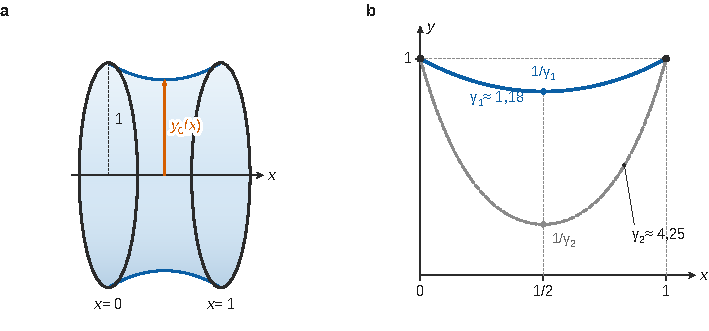
\includegraphics{figures/q18-profils-catenoide.pdf}
\caption*{Figure 4 --- (a) Caténoïde engendrée par la rotation du graphe de y₀
entre les cercles x = 0 et x = 1 ; (b) les deux profils ch(γ(x − 1/2))/γ
avec ch(γ/2) = γ}
\end{figure}

\end{document}
